\documentclass[a4paper,11pt,openany]{book}
\usepackage[utf8]{inputenc}
\usepackage[left=2.54cm,top=2.54cm,right=2.54cm,bottom=2.54cm]{geometry}
\usepackage[spanish]{babel}
\usepackage{amsmath}
\usepackage{amsfonts}
\usepackage{amssymb}
\usepackage{graphicx}
\usepackage{color}
\usepackage[usenames,dvipsnames]{xcolor}
\usepackage{pifont}
\usepackage{marvosym}
\newtheorem{teo}{Teorema}
\newtheorem{ejemplo}{Ejemplo}
\newtheorem{defi}{Definición}
\newtheorem{coro}{Corolario}
\newtheorem{prueba}{Prueba}
\newtheorem{exmp}{Example}[section]
\newtheorem{ejer}{Ejercicio}[section]
\def\proof{\paragraph{\textsf{Demostración.} }}
\def\endproof{\hfill $\blacksquare$ \\}
\usepackage{multirow, array} % para las tablas
\usepackage{multirow}
\usepackage{tabularx}
\usepackage{float} % para usar [H]
\usepackage{tikz}
\usepackage[all]{xy}
\usepackage{cancel}
\usetikzlibrary{positioning}
\usepackage{enumitem}
\newcommand*{\itembolasazules}[1]{% bolas 3D
\footnotesize\protect\tikz[baseline=-3pt]%
\protect\node[scale=.7, circle, shade, ball
color=green]{\color{white}\Large\bf#1};}
\usepackage{tcolorbox} 
\tcbuselibrary{listingsutf8}
\newtcolorbox[auto counter,number within=section]{example}[2][]
{colback=green!5!white,colframe=green!75!black,fonttitle=\bfseries, title=Ejercicio~\thetcbcounter: #2,#1}
\usepackage{background}
\backgroundsetup{
placement=center,
angle=0,
scale=1.1,
contents= {{
\includegraphics{HojaCuadriculada.png}}}
}
 
 
\begin{document}
\begin{titlepage}
 
\begin{center}
\vspace*{-1in}
\begin{figure}[htb]
\begin{center}

\includegraphics[width=7cm]{ETITC.png}
\end{center}
\end{figure}
 
 
{\sc \huge Escuela Tecnológica Instituto Técnico Central (ETITC)}\\
\vspace*{0.15in}
Facultad de sistemas\\
\vspace*{0.6in}
\begin{Large}
\textbf{Taller 2: Forma Polar, Potencias y Raíces de los Complejos} \\
\textbf{Matem{\'a}ticas Especiales}\\
\end{Large}
\vspace*{0.3in}
\begin{large}
{\bf Autores} \\
 
\ 
 
Sergio Alejandro Enrrique Caballero Leon\\ 
Johan Alejandro Sogamoso Camacho \\
David Andrés Valero Vanegas \\
\end{large}
\vspace*{0.3in}
 
\end{center}
 
\begin{center}
{\bf Presentado a:} \\
 
\ 
 
Carlos Romero \\
 
\
 
Bogot{\'a}, Septiembre de 2022.
\end{center}
 
\end{titlepage}

\newpage

\definecolor{ao(english)}{rgb}{0.0, 0.5, 0.0}

\graphicspath{ {images/} }

\begin{center}
\textbf{Multiplicación}
\end{center}

En cada uno de los ejercicios \textbf{(\,1\,)} al \textbf{(\,3\,)} realizar lo siguiente:\\

\textbf{a\,)} Calcular el producto de los números complejos $\bf{z_{1}\,\cdot\,z_{2}}$, usando la fórmula de la multiplicación en forma polar.\\

\textbf{b\,)} Escriba \textbf{el resultado del producto} en la forma cartesiana $\bf{z\,=\,x\,+\,i\,y}$ y en la forma exponencial $\bf{z\,=\,r\,e^{i\,\theta}}$ ó $\bf{z\,=\,r\,exp\,(i\,\theta)}$.\\

\textbf{c\,)} Realizar en un plano complejo la gráfica de $\bf{z_{1}}$, $\bf{z_{2}}$ y $\bf{z_{1}\,\cdot\,z_{2}}$.\\

\textcolor{ao(english)}{(\,1\,)} $\bf{z_{1}\,=\,4\,-\,4\,i \quad;\quad z_{2}\,=\,6\,-\,i\,6\,\sqrt{3}}$\\

\textcolor{ao(english)}{a\,)} Calcule $\bf{z_{1}\,\cdot\,z_{2}}$ en forma polar:

$$z_{1}\,\cdot\,z_{2}\,=\,r_{1}\,\cdot\,r_{2}\,\left[\cos\,(\theta_{1}\,+\,\theta_{2})\,+\,i\,\sin\,(\theta_{1}\,+\,\theta_{2})\right]$$

\textcolor{ao(english)}{\ding{47}} Forma polar de $\bf{z_{1}}$ y $\bf{z_{2}}$.\\

\textcolor{ao(english)}{\ding{46}} Módulo y ángulo de $\bf{z_{1}}$ 

$$r_{1}\,=\,|z_{1}|\,=\,\sqrt{(4)^{2}\,+\,(-\,4)^{2}}\,=\,\sqrt{16\,+\,16}\,=\,\sqrt{32}\,=\,4\,\sqrt{2}$$

$$\theta_{1}\,=\,\tan^{-\,1}\,\left(\dfrac{-\,4}{4}\right)\,=\,\tan^{-\,1}\,(-\,1)\,=\,-\,\dfrac{\pi}{4}$$

$$\boxed{r_{1}\,=\,4\,\sqrt{2} \quad;\quad \theta_{1}\,=\,-\,\dfrac{\pi}{4}}$$

\textcolor{ao(english)}{\ding{46}} Módulo y ángulo de $\bf{z_{2}}$ 

$$r_{2}\,=\,|z_{2}|\,=\,\sqrt{(6)^{2}\,+\,\left(-\,6\,\sqrt{3}\right)^{2}}\,=\,\sqrt{36\,+\,36(3)}\,=\,\sqrt{36\,+\,108}\,=\sqrt{144}\,=\,12$$

$$\theta_{2}\,=\,\tan^{-\,1}\,\left(\dfrac{-\,6\,\sqrt{3}}{6}\right)\,=\,\tan^{-\,1}\,(-\,\sqrt{3})\,=\,-\,\dfrac{\pi}{3}$$

$$\boxed{r_{2}\,=\,12 \quad;\quad \theta_{2}\,=\,-\,\dfrac{\pi}{3}}$$

\textcolor{ao(english)}{\ding{47}} Calcular $\bf{z_{1}\,\cdot\,z_{2}}$

$$z_{3}\,=\,z_{1}\,\cdot\,z_{2}$$

$$z_{3}\,=\,\left(4\,\sqrt{2}\right)\,(12)\,\left[\cos\,\left(-\,\dfrac{\pi}{4}\,+\,\left(-\,\dfrac{\pi}{3}\right)\right)\,+\,i\,\sin\,\left(-\,\dfrac{\pi}{4}\,+\,\left(-\,\dfrac{\pi}{3}\right)\right)\right]$$

$$=\,48\,\sqrt{2}\,\left[\cos\,\left(-\,\dfrac{\pi}{4}\,-\,\dfrac{\pi}{3}\right)\,+\,i\,\sin\,\left(-\,\dfrac{\pi}{4}\,-\,\dfrac{\pi}{3}\right)\right]$$

$$=\,48\,\sqrt{2}\,\left[\cos\,\left(\dfrac{-\,3\pi\,-\,4\,\pi}{12}\right)\,+\,i\,\sin\,\left(\dfrac{-\,3\,\pi\,-\,4\,\pi}{12}\right)\right]$$

$$z_{3}\,=\,48\,\sqrt{2}\,\left[\cos\,\left(-\,\dfrac{7\,\pi}{12}\right)\,+\,i\,\sin\,\left(-\,\dfrac{7\,\pi}{12}\right)\right]$$

\textcolor{ao(english)}{b\,)} Formas cartesiana y exponenccial $\bf{z_{3}}$\\

\textcolor{ao(english)}{\ding{47}} Cartesiana

$$x\,=\,48\,\sqrt{2}\,\cos\,\left(-\,\dfrac{7\,\pi}{12}\right)\,\approx\,-\,17.57$$

$$y\,=\,48\,\sqrt{2}\,\sin\,\left(-\,\dfrac{7\pi}{12}\right)\,\approx\,-\,65.57$$

$$z_{3}\,=\,-\,17.57\,-\,65.57\,i$$

\textcolor{ao(english)}{\ding{47}} Exponencial

$$z_{3}\,=\,48\,\sqrt{2}\,\cdot\,exp\,\left(-\,\dfrac{7\,\pi}{12}\,i\right)$$

\textcolor{ao(english)}{c\,)} Graficar plano complejo\\

\textcolor{ao(english)}{\ding{47}} Gráfica $\bf{z_{1}}$ y $\bf{z_{2}}$

\begin{center}
    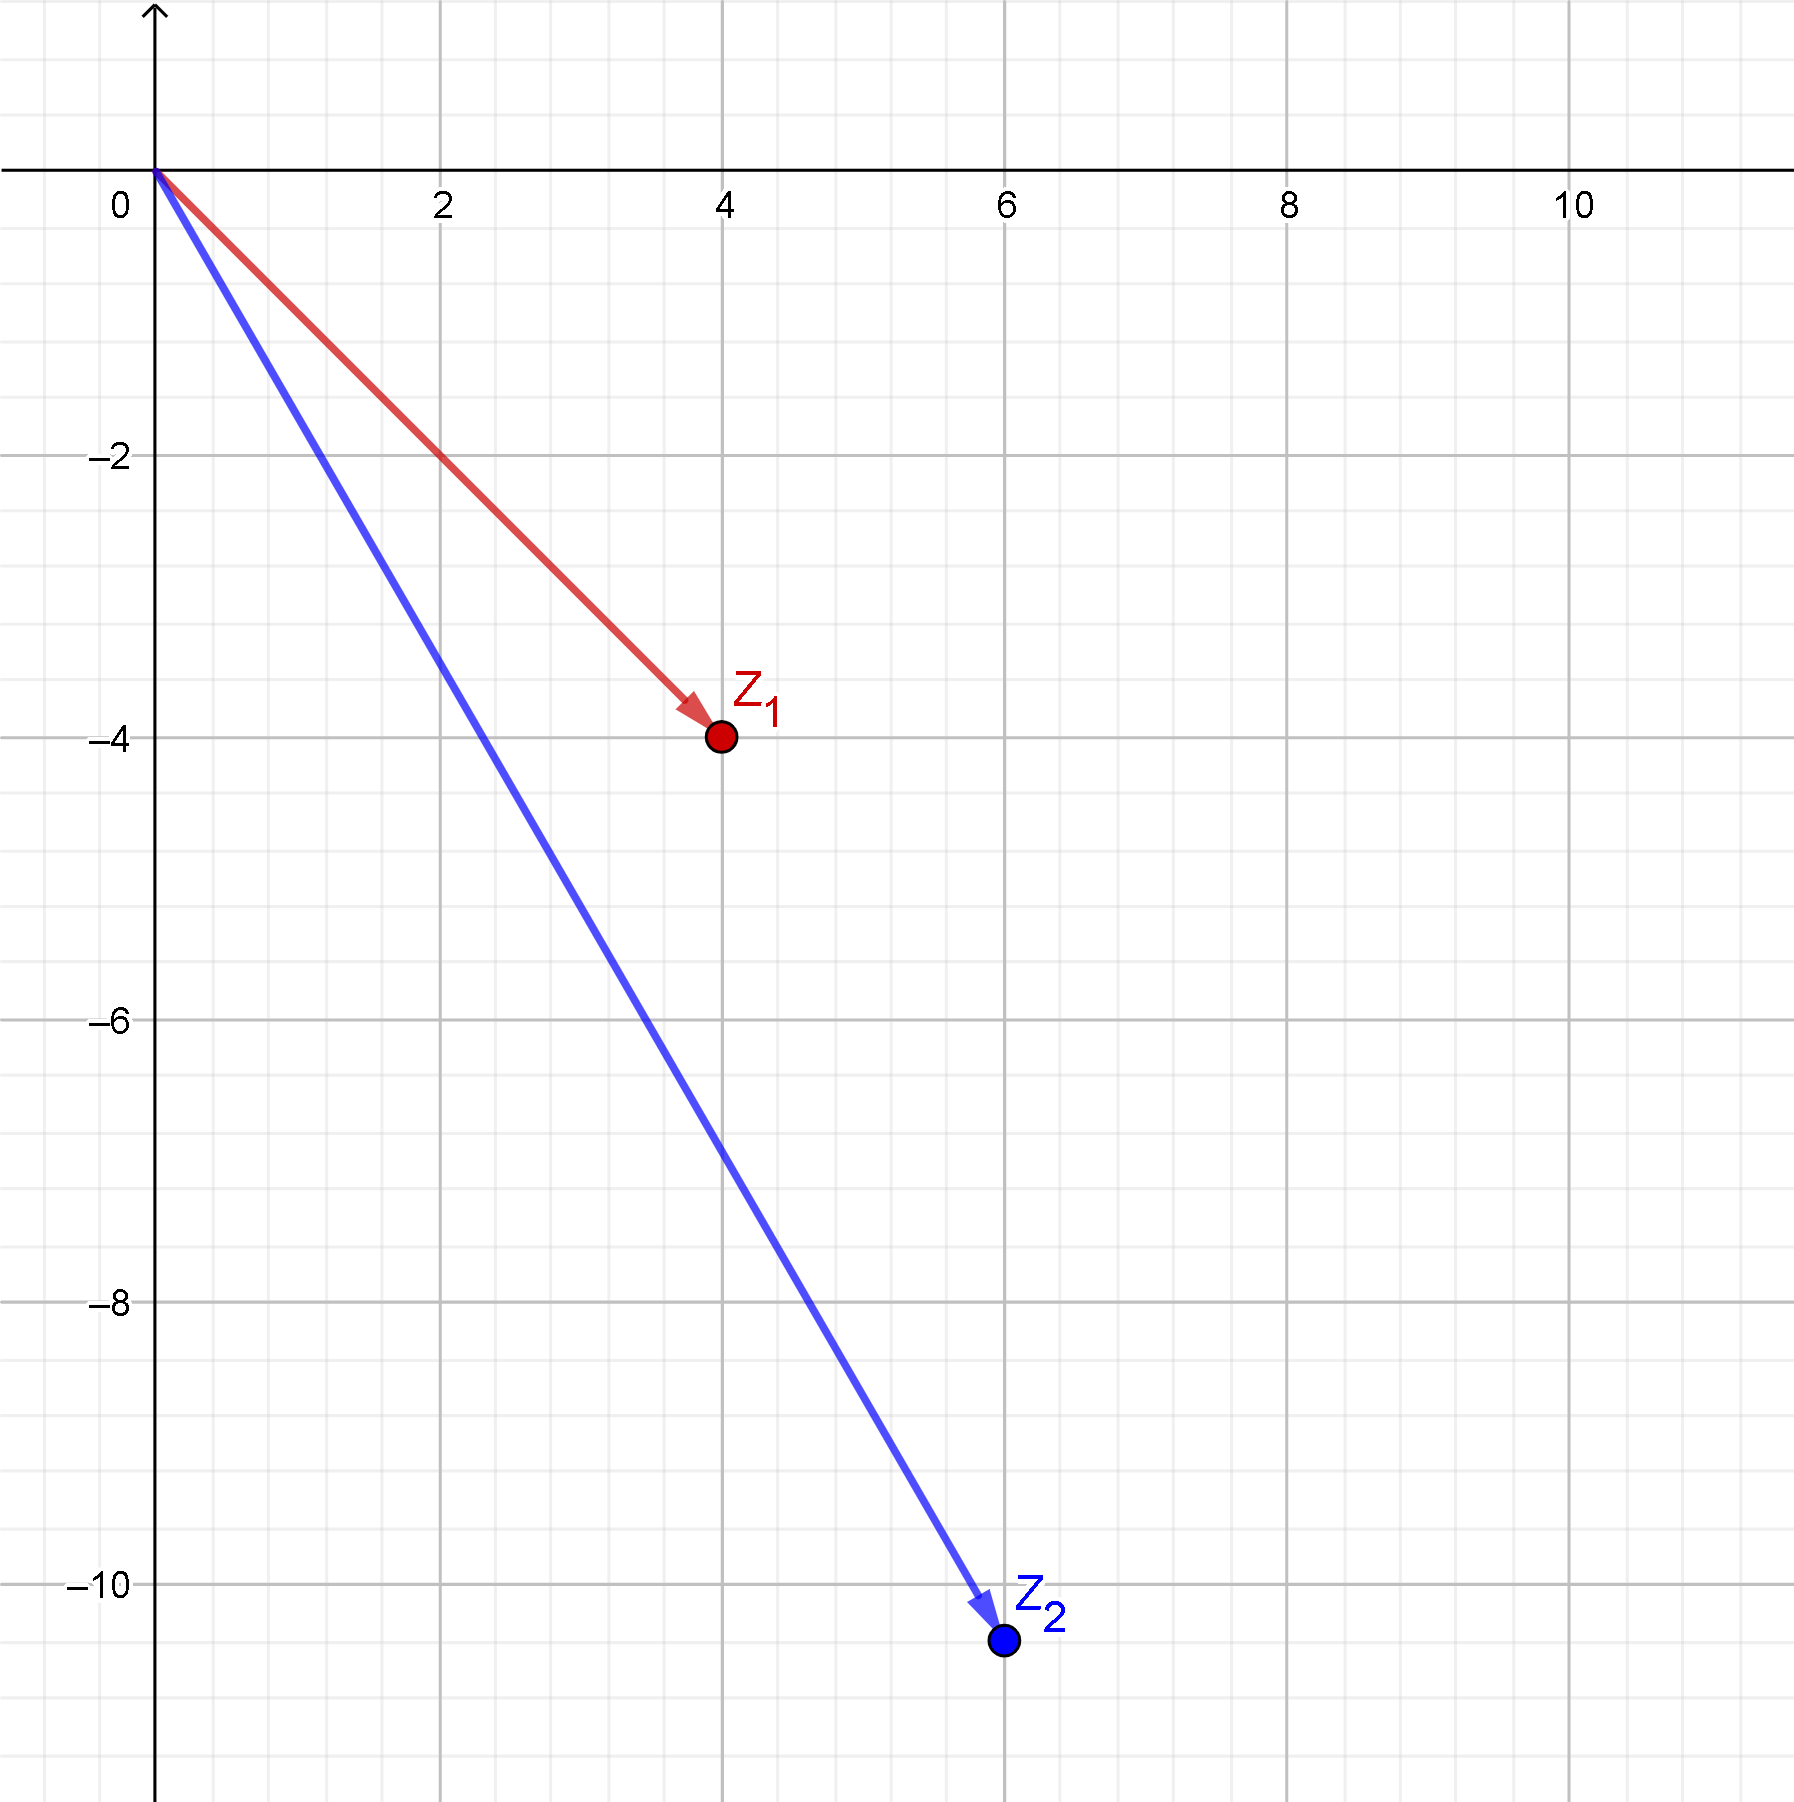
\includegraphics[width=10cm]{Gra-Ej-1-1.png}
\end{center}

\newpage

\textcolor{ao(english)}{\ding{47}} Gráfica $\bf{z_{3}\,=\,z_{1}\,\cdot\,z_{2}}$

\begin{center}
    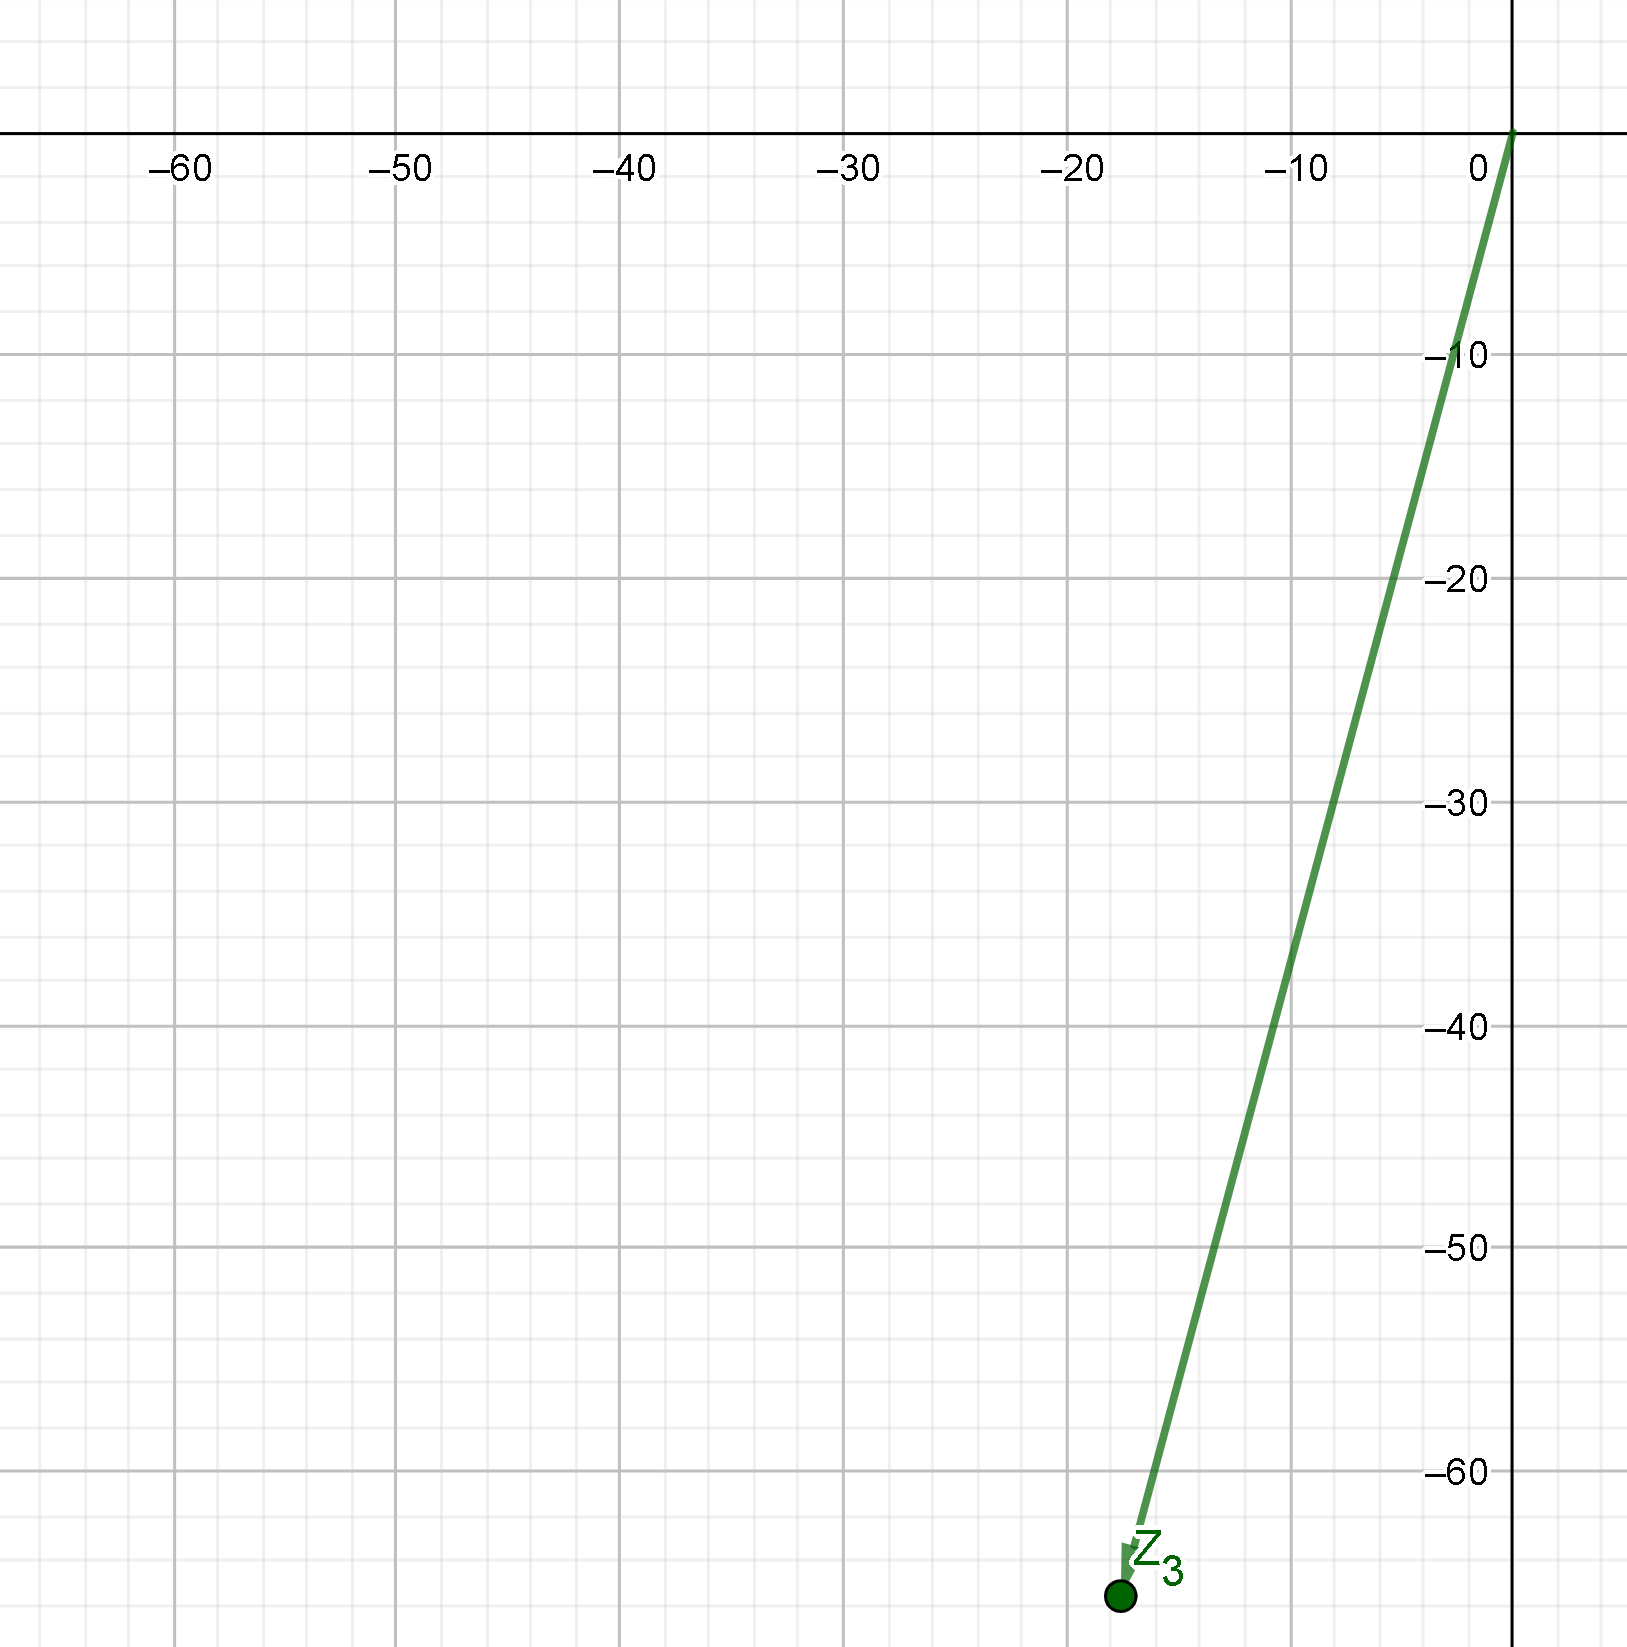
\includegraphics[width=10cm]{Gra-Ej-1-2.png}
\end{center}

\textcolor{ao(english)}{(\,2\,)} $\bf{z_{1}\,=\,2\,-\,i \quad;\quad z_{2}\,=\,-\,2\,+\,2\,i}$

\textcolor{ao(english)}{(\,3\,)} $\bf{z_{1}\,=\,1\,-\,i \quad;\quad z_{2}\,=\,1\,-\,i\,\sqrt{3}}$\\



\textcolor{ao(english)}{a\,)} Calcule $\bf{z_{1}\,\cdot\,z_{2}}$ en forma polar:

$$z_{1}\,\cdot\,z_{2}\,=\,r_{1}\,\cdot\,r_{2}\,\left[\cos\,(\theta_{1}\,+\,\theta_{2})\,+\,i\,\sin\,(\theta_{1}\,+\,\theta_{2})\right]$$

\textcolor{ao(english)}{\ding{47}} Forma polar de $\bf{z_{1}}$ y $\bf{z_{2}}$.\\

\textcolor{ao(english)}{\ding{46}} Módulo y ángulo de $\bf{z_{1}}$ 

$$r_{1}\,=\,|z_{1}|\,=\,\sqrt{(1)^{2}\,+\,(-\,1)^{2}}\,=\,\sqrt{1\,+\,1}\,=\,\sqrt{2}$$

$$\theta_{1}\,=\,\tan^{-\,1}\,\left(\dfrac{-\,1}{1}\right)\,=\,\tan^{-\,1}\,(-\,1)\,=\,-\,\dfrac{\pi}{4}$$

$$\boxed{r_{1}\,=\,\sqrt{2} \quad;\quad \theta_{1}\,=\,-\,\dfrac{\pi}{4}}$$

\textcolor{ao(english)}{\ding{46}} Módulo y ángulo de $\bf{z_{2}}$ 

$$r_{2}\,=\,|z_{2}|\,=\,\sqrt{(1)^{2}\,+\,\left(-\,\sqrt{3}\right)^{2}}\,=\,\sqrt{1\,+\,3}\,=\,\sqrt{4\,}=\,2$$

$$\theta_{2}\,=\,\tan^{-\,1}\,\left(\dfrac{-\,\sqrt{3}}{1}\right)\,=\,\tan^{-\,1}\,(-\,\sqrt{3})\,=\,-\,\dfrac{\pi}{3}$$

$$\boxed{r_{2}\,=\,2 \quad;\quad \theta_{2}\,=\,-\,\dfrac{\pi}{3}}$$

\textcolor{ao(english)}{\ding{47}} Calcular $\bf{z_{1}\,\cdot\,z_{2}}$

$$z_{3}\,=\,z_{1}\,\cdot\,z_{2}$$

$$z_{3}\,=\,\left(2\,\sqrt{2}\right)\,\left[\cos\,\left(-\,\dfrac{\pi}{4}\,+\,\left(-\,\dfrac{\pi}{3}\right)\right)\,+\,i\,\sin\,\left(-\,\dfrac{\pi}{4}\,+\,\left(-\,\dfrac{\pi}{3}\right)\right)\right]$$

$$=\,2\,\sqrt{2}\,\left[\cos\,\left(-\,\dfrac{\pi}{4}\,-\,\dfrac{\pi}{3}\right)\,+\,i\,\sin\,\left(-\,\dfrac{\pi}{4}\,-\,\dfrac{\pi}{3}\right)\right]$$

$$=\,2\,\sqrt{2}\,\left[\cos\,\left(\dfrac{-\,3\pi\,-\,4\,\pi}{12}\right)\,+\,i\,\sin\,\left(\dfrac{-\,3\,\pi\,-\,4\,\pi}{12}\right)\right]$$

$$z_{3}\,=\,2\,\sqrt{2}\,\left[\cos\,\left(-\,\dfrac{7\,\pi}{12}\right)\,+\,i\,\sin\,\left(-\,\dfrac{7\,\pi}{12}\right)\right]$$

\textcolor{ao(english)}{b\,)} Formas cartesiana y exponenccial $\bf{z_{3}}$\\

\textcolor{ao(english)}{\ding{47}} Cartesiana

$$x\,=\,2\,\sqrt{2}\,\cos\,\left(-\,\dfrac{7\,\pi}{12}\right)\,\approx\,-\,0.73$$

$$y\,=\,2\,\sqrt{2}\,\sin\,\left(-\,\dfrac{7\pi}{12}\right)\,\approx\,-\,2.73$$

$$z_{3}\,=\,-\,0.73\,-\,2.73\,i$$

\textcolor{ao(english)}{\ding{47}} Exponencial

$$z_{3}\,=\,2\,\sqrt{2}\,\cdot\,exp\,\left(-\,\dfrac{7\,\pi}{12}\,i\right)$$

\textcolor{ao(english)}{c\,)} Graficar plano complejo\\

\textcolor{ao(english)}{\ding{47}} Gráfica $\bf{z_{1}}$ y $\bf{z_{2}}$

\begin{center}
    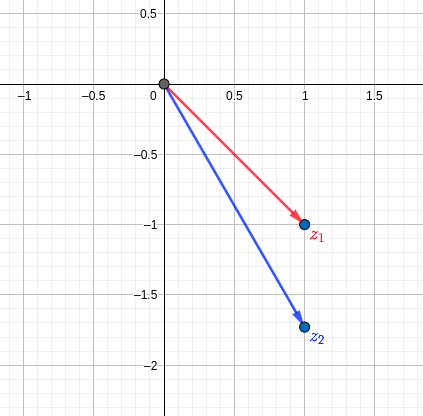
\includegraphics[width=10cm]{Gra-Ej-3-1.png}
\end{center}

\newpage

\textcolor{ao(english)}{\ding{47}} Gráfica $\bf{z_{3}\,=\,z_{1}\,\cdot\,z_{2}}$

\begin{center}
    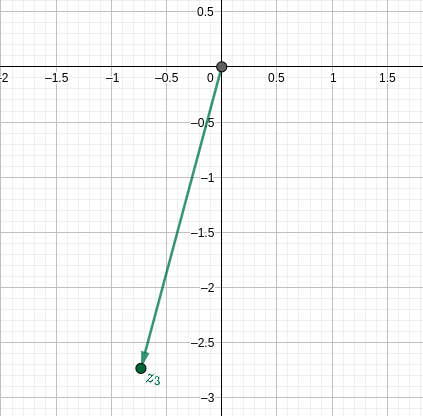
\includegraphics[width=10cm]{Gra-Ej-3-2.png}
\end{center}




\begin{center}
\textbf{División}
\end{center}

En cada uno de los ejercicios \textbf{(\,4\,)} al \textbf{(\,6\,)} realizar lo siguiente:\\

\textbf{a\,)} Calcule $\bf{z_{1}\,\div\,z_{2}}$, usando la fórmula de la división en forma polar.\\

\textbf{b\,)} Escriba \textbf{el resultado de la división} en la forma cartesiana $\bf{z\,=\,x\,+\,i\,y}$ y en la forma exponencial $\bf{z\,=\,r\,e^{i\,\theta}}$ ó $\bf{z\,=\,r\,exp\,(i\,\theta)}$.\\

\textbf{c\,)} Realizar en un plano complejo la gráfica de $\bf{z_{1}}$, $\bf{z_{2}}$ y $\bf{z_{1}\,\div\,z_{2}}$.\\

\textcolor{ao(english)}{(\,4\,)} $\bf{z_{1}\,=\,2\,-\,2\,i \quad;\quad z_{2}\,=\,3\,-\,i\,3\,\sqrt{3}}$

\textcolor{ao(english)}{(\,5\,)} $\bf{z_{1}\,=\,-\,1\,-\,i\,\sqrt{3} \quad;\quad z_{2}\,=\,-\,4\,+\,4\,i}$

\textcolor{ao(english)}{a\,)} Calcule $\bf{z_{1}\,\div\,z_{2}}$ en forma polar:

$$\dfrac{z_{1}}{z_{2}}\,=\,\dfrac{r_{1}}{r_{2}}\,\left[\cos\,(\theta_{1}\,-\,\theta_{2})\,+\,i\,\sin\,(\theta_{1}\,-\,\theta_{2})\right]$$

\textcolor{ao(english)}{\ding{47}} Forma polar de $\bf{z_{1}}$ y $\bf{z_{2}}$.\\

\textcolor{ao(english)}{\ding{46}} Módulo y ángulo de $\bf{z_{1}}$ 

$$r_{1}\,=\,|z_{1}|\,=\,\sqrt{(-\,1)^{2}\,+\,(-\,\sqrt{3})^{2}}\,=\,\sqrt{1\,+\,3}\,=\,\sqrt{4}\,=\,2$$

$$\theta_{0}\,=\,\tan^{-\,1}\,\left(\dfrac{-\,\sqrt{3}}{-\,1}\right)\,=\,\tan^{-\,1}\,(\sqrt{3})\,=\,\dfrac{\pi}{3}$$

\textcolor{ao(english)}{\ding{43}} Correción $\theta_{0}$ Cuadrantre III

$$\theta_{1}\,=\,|\theta_{0}|\,-\,\pi\,=\,\left|\dfrac{\pi}{3}\right|\,-\,\pi\,=\,\dfrac{\pi}{3}\,-\,\pi\,=\,\dfrac{\pi\,-\,3\,\pi}{3}\,=\,-\,\dfrac{2\,\pi}{3}$$

$$\boxed{r_{1}\,=\,2 \quad;\quad \theta_{1}\,=\,-\,\dfrac{2\,\pi}{3}}$$

\textcolor{ao(english)}{\ding{46}} Módulo y ángulo de $\bf{z_{2}}$ 

$$r_{2}\,=\,|z_{2}|\,=\,\sqrt{(-\,4)^{2}\,+\,(4)^{2}}\,=\,\sqrt{16\,+\,16}\,=\,\sqrt{32}\,=\,4\,\sqrt{2}$$

$$\theta_{0}\,=\,\tan^{-\,1}\,\left(\dfrac{4}{-\,4}\right)\,=\,\tan^{-\,1}\,(-\,1)\,=\,-\,\dfrac{\pi}{4}$$

\textcolor{ao(english)}{\ding{43}} Correción $\theta_{0}$ Cuadrantre II

$$\theta_{2}\,=\,\pi\,-\,|\theta_{0}|\,=\,\pi\,-\,\left|-\,\dfrac{\pi}{4}\right|\,=\,\pi\,-\,\dfrac{\pi}{4}\,=\,\dfrac{4\,\pi\,-\,\pi}{4}\,=\,\dfrac{3\,\pi}{4}$$

$$\boxed{r_{2}\,=\,4\,\sqrt{2} \quad;\quad \theta_{2}\,=\,\dfrac{3\,\pi}{4}}$$

\textcolor{ao(english)}{\ding{47}} Calcular $\bf{z_{1}\,\div\,z_{2}}$

$$z_{3}\,=\,\dfrac{z_{1}}{z_{2}}$$

$$z_{3}\,=\,\dfrac{2}{4\,\sqrt{2}}\,\left[\cos\,\left(-\,\dfrac{2\,\pi}{3}\,-\,\dfrac{3\,\pi}{4}\right)\,+\,i\,\sin\,\left(-\,\dfrac{2\,\pi}{3}\,-\,\dfrac{3\,\pi}{4}\right)\right]$$

$$=\,\dfrac{1}{2\,\sqrt{2}}\,\left[\cos\,\left(\dfrac{-\,9\,\pi\,-\,8\,\pi}{12}\right)\,+\,i\,\sin\,\left(\dfrac{-\,9\,\pi\,-\,8\,\pi}{12}\right)\right]$$

$$z_{3}\,=\,\dfrac{1}{2\,\sqrt{2}}\,\left[\cos\,\left(-\,\dfrac{17\,\pi}{12}\right)\,+\,i\,\sin\,\left(-\,\dfrac{17\,\pi}{12}\right)\right]$$

\textcolor{ao(english)}{b\,)} Formas cartesiana y exponenccial $z_{3}$\\

\textcolor{ao(english)}{\ding{47}} Cartesiana

$$x\,=\,\dfrac{1}{2\,\sqrt{2}}\,\cos\,\left(-\,\dfrac{17\,\pi}{12}\right)\,\approx\,-\,0.1$$

$$y\,=\,\dfrac{1}{2\,\sqrt{2}}\,\sin\,\left(-\,\dfrac{17\pi}{12}\right)\,\approx\,0.34$$

$$z_{3}\,=\,-\,0.1\,+\,0.34\,i$$

\textcolor{ao(english)}{\ding{47}} Exponencial

$$z_{3}\,=\,\dfrac{1}{2\,\sqrt{2}}\,\cdot\,exp\,\left(-\,\dfrac{17\,\pi}{12}\,i\right)$$

\textcolor{ao(english)}{c\,)} Graficar plano complejo\\

\textcolor{ao(english)}{\ding{47}} Gráfica $\bf{z_{1}}$ y $\bf{z_{2}}$

\begin{center}
    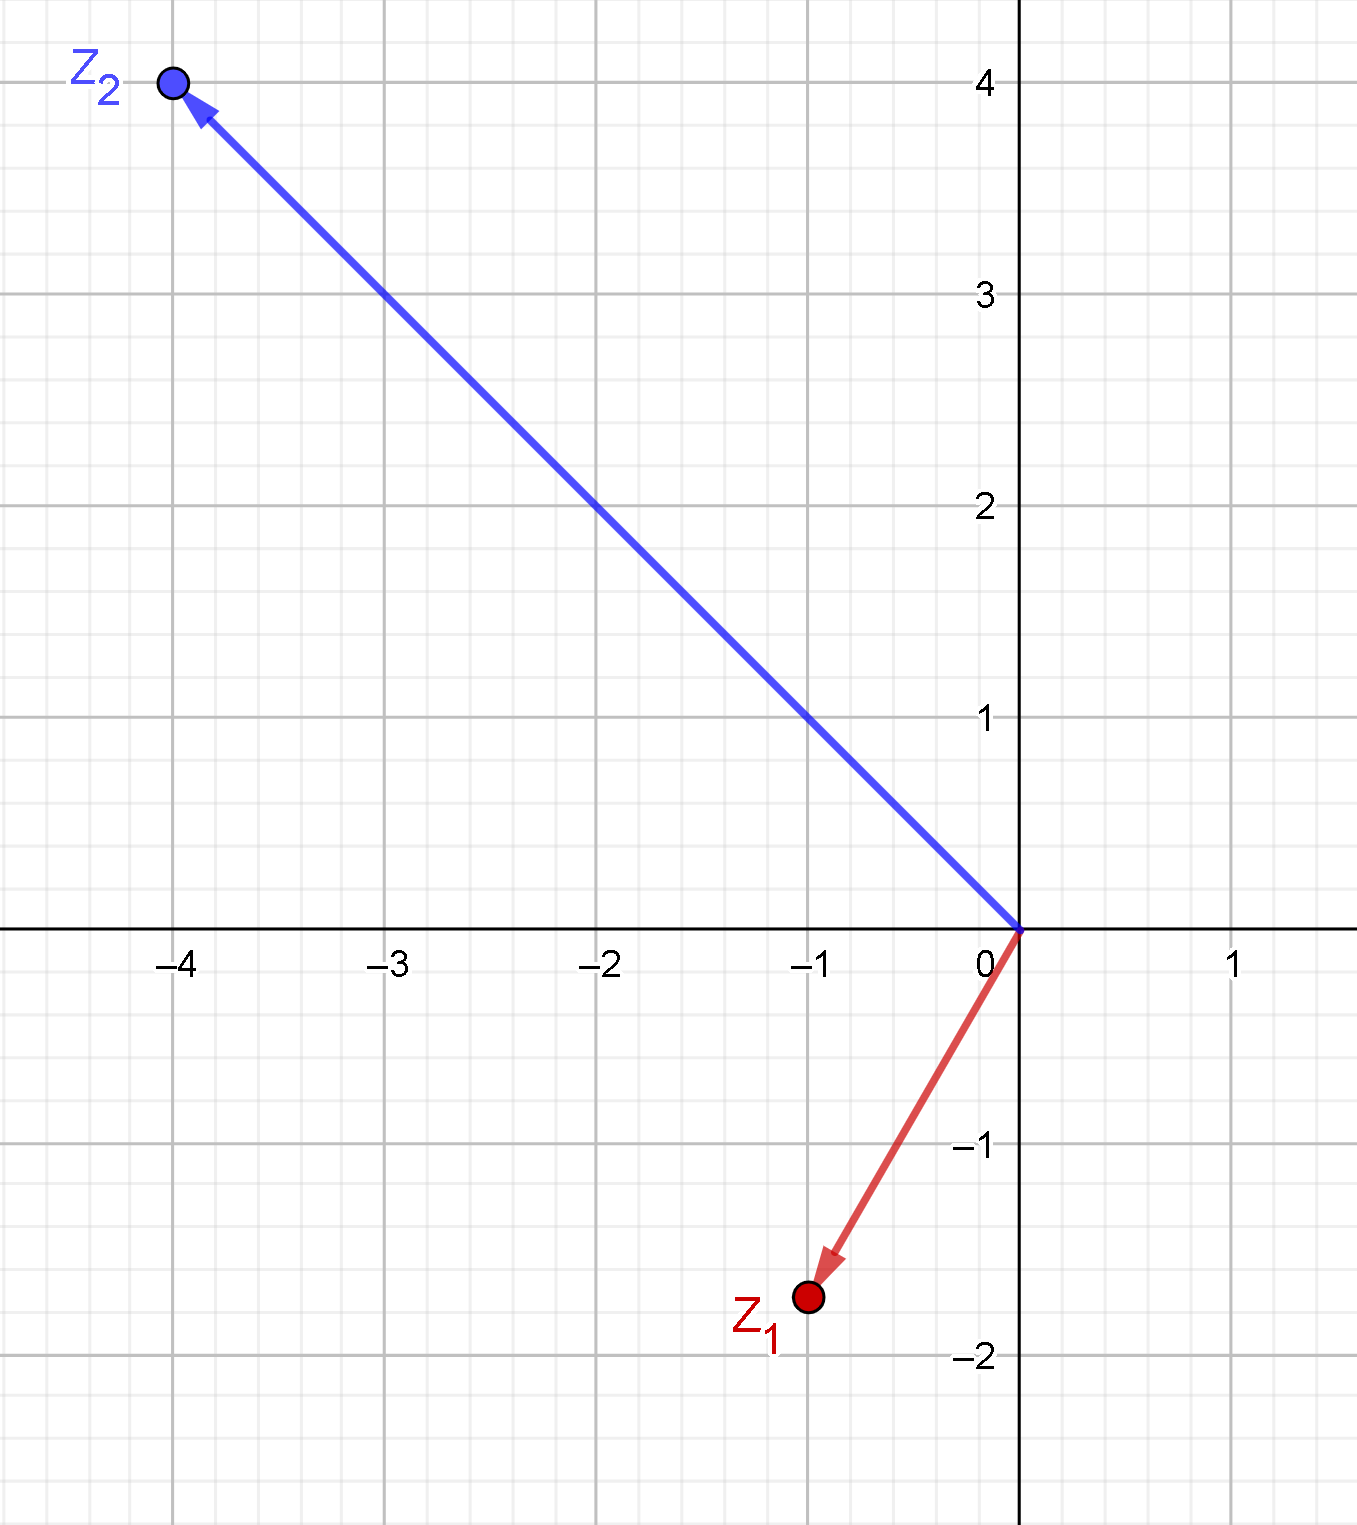
\includegraphics[width=10cm]{Gra-Ej-5-1.png}
\end{center}

\textcolor{ao(english)}{\ding{47}} Gráfica $\bf{z_{3}\,=\,z_{1}\,\div\,z_{2}}$

\begin{center}
    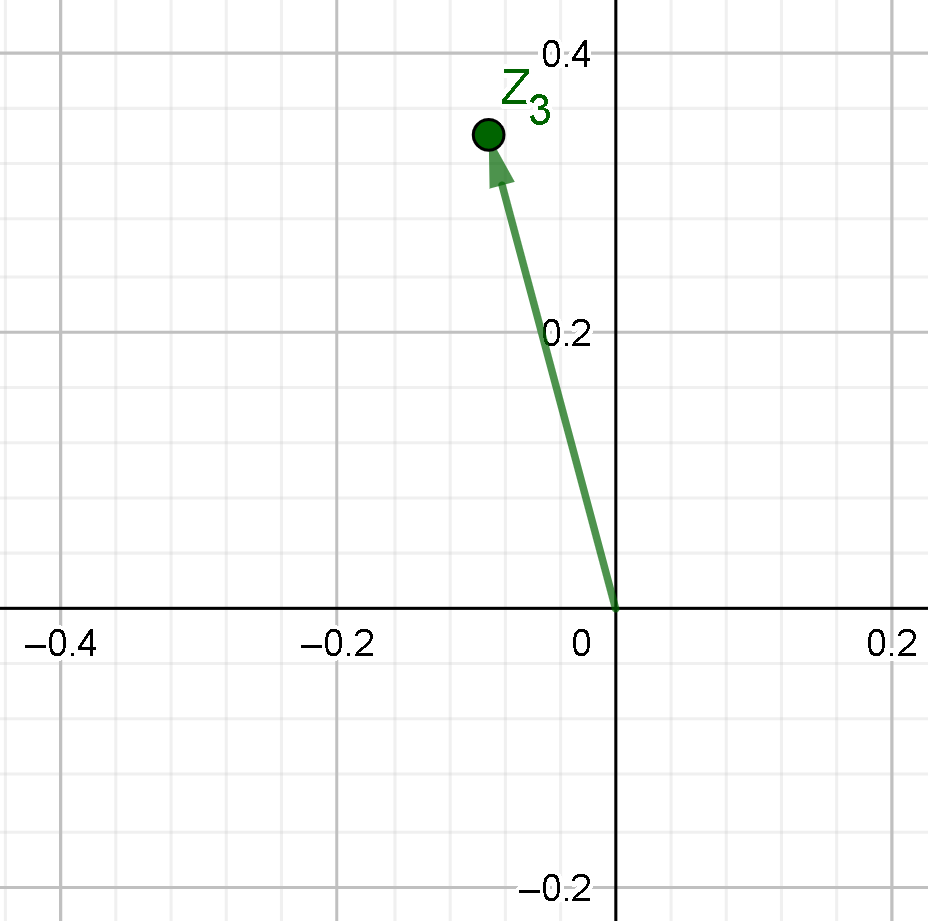
\includegraphics[width=10cm]{Gra-Ej-5-2.png}
\end{center}

\textcolor{ao(english)}{(\,6\,)} $\bf{z_{1}\,=\,2\,-\,2\,i \quad;\quad z_{2}\,=\,2\,-\,i\,2\,\sqrt{3}}$


\textcolor{ao(english)}{a\,)} Calcule $\bf{z_{1}\,\div\,z_{2}}$ en forma polar

$$\dfrac{z_{1}}{z_{2}}\,=\,\dfrac{r_{1}}{r_{2}}\,\left[\cos\,(\theta_{1}\,-\,\theta_{2})\,+\,i\,\sin\,(\theta_{1}\,-\,\theta_{2})\right]$$

\textcolor{ao(english)}{\ding{47}} Forma polar de $\bf{z_{1}}$ y $\bf{z_{2}}$.\\

\textcolor{ao(english)}{\ding{46}} Módulo y ángulo de $\bf{z_{1}}$ 

$$r_{1}\,=\,|z_{1}|\,=\,\sqrt{(2)^{2}\,+\,(-\,2)^{2}}\,=\,\sqrt{4\,+\,4}\,=\,\sqrt{8}\,=\,2\,\sqrt{2}\,\approx\,2.83$$

$$\theta_{0}\,=\,\tan^{-\,1}\,\left(\dfrac{-\,2}{2}\right)\,=\,\tan^{-\,1}\,(-\,1)\,=\,-\,\dfrac{\pi}{4}$$

$$\boxed{r_{1}\,=\,2\,\sqrt{2}\, \quad;\quad \theta_{1}\,=\,-\,\dfrac{\pi}{4}}$$

\textcolor{ao(english)}{\ding{46}} Módulo y ángulo de $\bf{z_{2}}$ 

$$r_{2}\,=\,|z_{2}|\,=\,\sqrt{(2)^{2}\,+\,(\,-\,2\,\sqrt{3})^{2}}\,=\,\sqrt{4\,+\,12}\,=\,\sqrt{16}\,=\,4$$

$$\theta_{0}\,=\,\tan^{-\,1}\,\left(\dfrac{-\,2\,\sqrt{3}}{2}\right)\,=\,\tan^{-\,1}\,(-\,\sqrt{3})\,=\,-\,\dfrac{\pi}{3}$$

$$\boxed{r_{2}\,=\,4 \quad;\quad \theta_{2}\,=\,-\,\dfrac{\pi}{3}}$$

\textcolor{ao(english)}{\ding{47}} Calcular $\bf{z_{1}\,\div\,z_{2}}$

$$z_{3}\,=\,\dfrac{z_{1}}{z_{2}}$$

$$z_{3}\,=\,\dfrac{\,2\,\sqrt{2}\,}{4}\,\left[\cos\,\left(-\,\dfrac{\pi}{4}\,-\,\left(-\,\dfrac{\pi}{3}\right)\right)\,+\,i\,\sin\,\left(-\,\dfrac{\pi}{4}\,-\,\left(-\,\dfrac{\pi}{3}\right)\right)\right]$$

$$z_{3}\,=\,\dfrac{\,\sqrt{2}\,}{2}\,\left[\cos\,\left(-\,\dfrac{\pi}{4}\,+\,\dfrac{\pi}{3}\right)\,+\,i\,\sin\,\left(-\,\dfrac{\pi}{4}\,+\,\dfrac{\pi}{3}\right)\right]$$

$$z_{3}\,=\,\dfrac{\,\sqrt{2}\,}{2}\,\left[\cos\,\left(\,\dfrac{\pi}{12}\,\right)\,+\,i\,\sin\,\left(\,\dfrac{\pi}{12}\,\right)\right]$$

\textcolor{ao(english)}{b\,)} Formas cartesiana y exponenccial $z_{3}$\\

\textcolor{ao(english)}{\ding{47}} Cartesiana

$$x\,=\,\dfrac{\sqrt{2}}{2}\,\cos\,\left(\dfrac{\pi}{12}\right)\,\approx\,0.68$$

$$y\,=\,\dfrac{\sqrt{2}}{2}\,\sin\,\left(\dfrac{\pi}{12}\right)\,\approx\,0.18$$

$$z_{3}\,=\,0.68\,+\,0.18\,i$$

\textcolor{ao(english)}{\ding{47}} Exponencial

$$z_{3}\,=\,\dfrac{\sqrt{2}}{2}\,\cdot\,exp\,\left(\dfrac{\pi}{12}\,i\right)$$

\textcolor{ao(english)}{c\,)} Graficar plano complejo\\

\textcolor{ao(english)}{\ding{47}} Gráfica $\bf{z_{1}}$ y $\bf{z_{2}}$

\begin{center}
    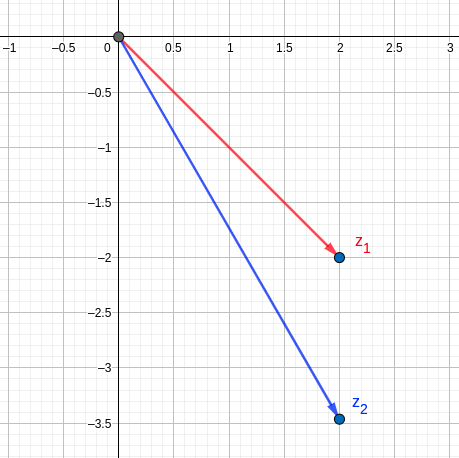
\includegraphics[width=10cm]{Gra-Ej-6-1.png}
\end{center}

\textcolor{ao(english)}{\ding{47}} Gráfica $\bf{z_{3}\,=\,z_{1}\,\div\,z_{2}}$

\begin{center}
    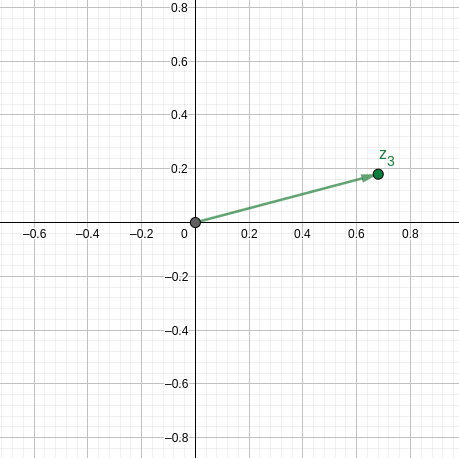
\includegraphics[width=10cm]{Gra-Ej-6-2.png}
\end{center}

\begin{center}
\textbf{Potencias Enteras de Números Complejos}
\end{center}

En cada uno de los ejercicios \textbf{(\,7\,)} al \textbf{(\,8\,)} realizar lo siguiente:\\

\textbf{a\,)} Calcule las potencias indicadas en forma exponencial.\\

\textbf{b\,)} Escriba el resultado final en la forma cartesiana $\bf{z^{n}\,=\,x\,+\,i\,y}$.\\

\textbf{c\,)} Dibujo en uno dos planos complejos los números, $\bf{z}$ y $\bf{z^{n}}$.\\

\textcolor{ao(english)}{(\,7\,)} $\bf{\left(1\,+\,i\,\sqrt{3}\right)^{9}}$

\textcolor{ao(english)}{a\,)} Potencia en forma exponnencial

$$z^{n}\,=\,r^{n}\,\cdot\,exp\,(i\,n\,\theta)$$

$$z\,=\,1\,+\,i\,\sqrt{3}$$

\textcolor{ao(english)}{\ding{47}} Hallar el módulo de \textbf{z}

$$r\,=\,|z|\,=\,\sqrt{(1)^{2}\,+\,\left(\sqrt{3}\right)^{2}}\,=\,\sqrt{1\,+\,3}\,=\,\sqrt{4}\,=\,2$$

\textcolor{ao(english)}{\ding{47}} Hallar el angulo de \textbf{z}

$$\theta\,=\,\tan^{-\,1}\,\sqrt{3}\,=\,\dfrac{\pi}{3}$$

\textcolor{ao(english)}{\ding{47}} Potencia donde $n\,=\,9$

$$z^{9}\,=\,2^{9}\,\cdot\,exp\,\left(i9\left(\dfrac{\pi}{3}\right)\right)$$

$$z^{9}\,=\,512\,\cdot\,exp\,\left(3\,\pi\,i\right)$$

\textcolor{ao(english)}{b\,)} Forma cartesina $\bf{z^{n}\,=\,x\,+\,i\,y}$

$$x\,=\,r\,\cos\,(\theta)\,=\,512\,\cos\,(3\,\pi)\,=\,-\,512$$

$$y\,=\,r\,\sin\,(\theta)\,=\,512\,\sin\,(3\,\pi)\,=\,0$$

$$z^{9}\,=\,-\,512$$

\textcolor{ao(english)}{c\,)} Graficar plano complejo\\

\textcolor{ao(english)}{\ding{47}} Gráfica $\bf{z}$

\begin{center}
    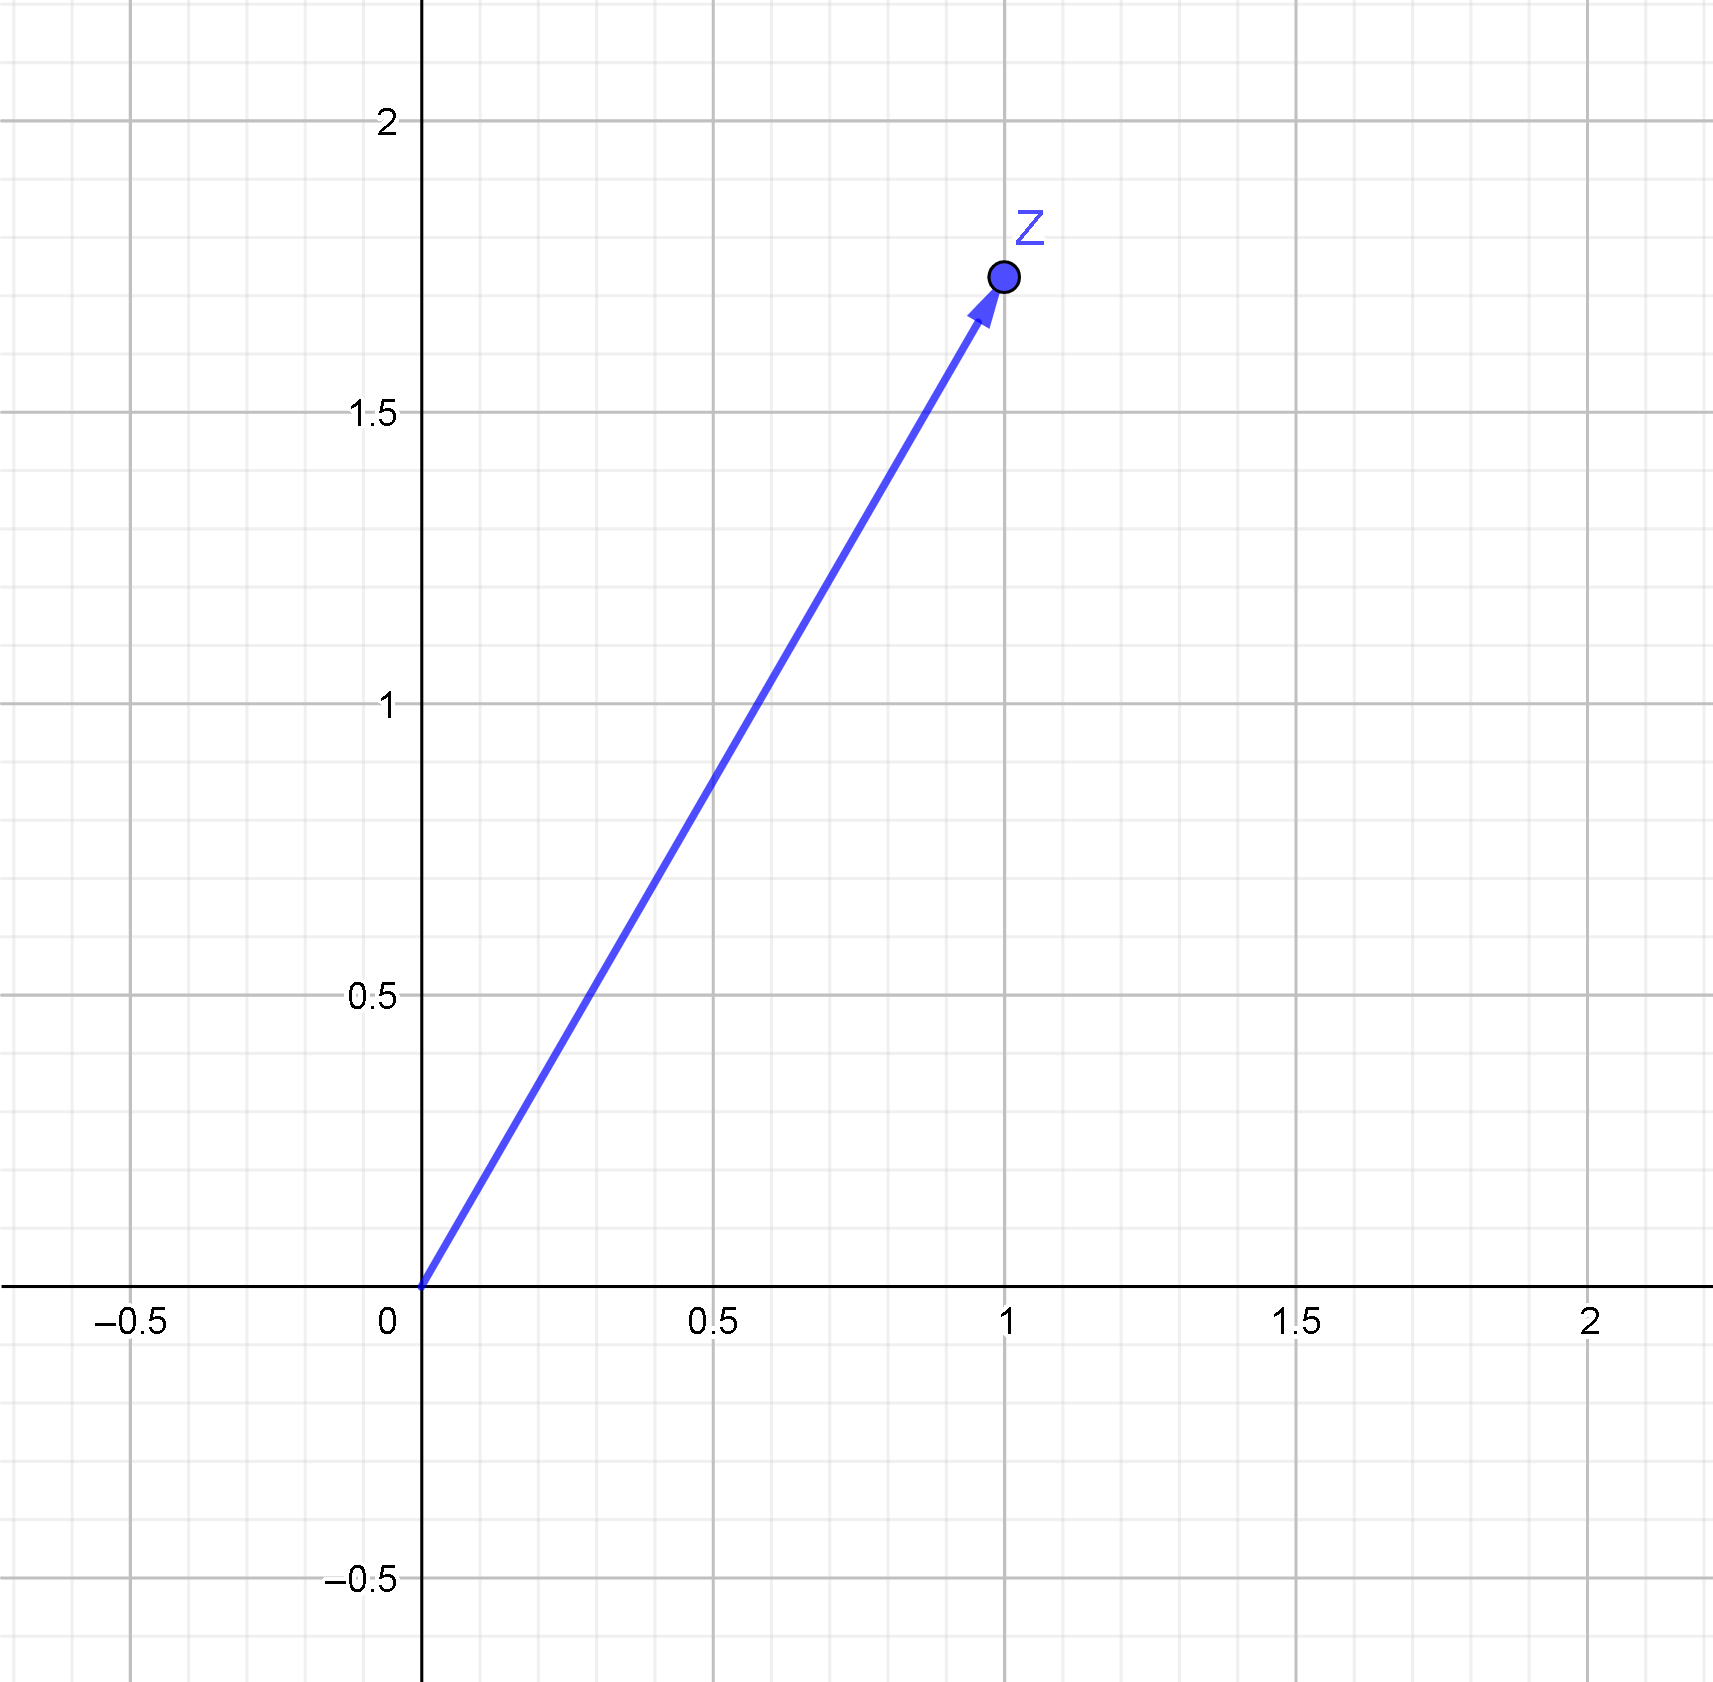
\includegraphics[width=10cm]{Gra-Ej-7-1.png}
\end{center}

\textcolor{ao(english)}{\ding{47}} Gráfica $\bf{z^{9}}$

\begin{center}
    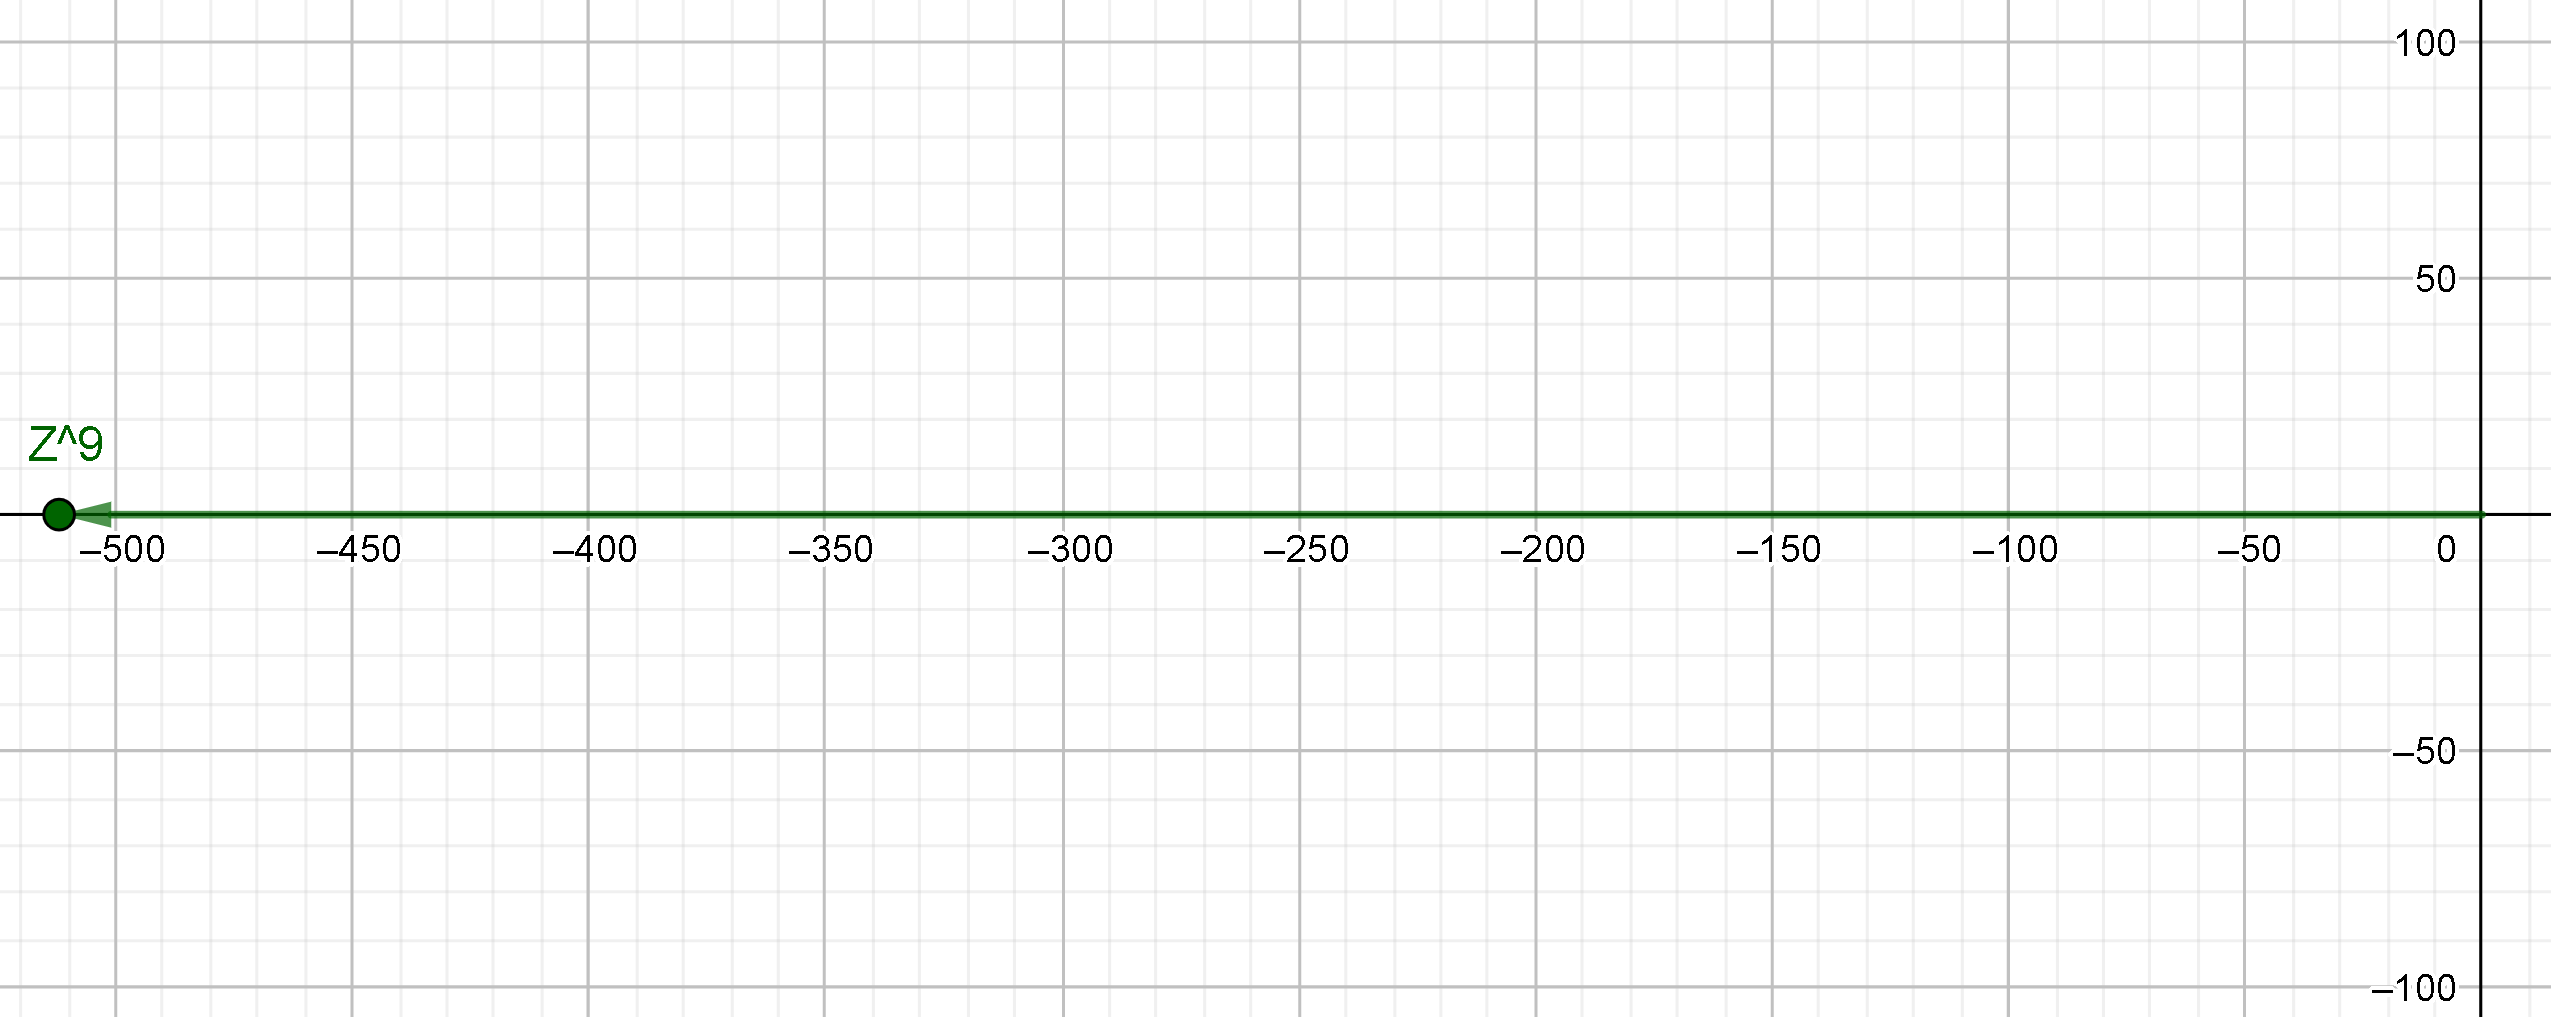
\includegraphics[width=15cm]{Gra-Ej-7-2.png}
\end{center}

\textcolor{ao(english)}{(\,8\,)} $\bf{\left(2\,-\,2\,i\right)^{5}}$

\begin{center}
\textbf{Raíces de Números Complejos}
\end{center}

Hallar las raíces indicadas a continuación y realizar su correspondiente gráfica en el plano complejo.\\

\textcolor{ao(english)}{(\,9\,)} $\bf{\sqrt[3]{8}}$\\


\textcolor{ao(english)}{\ding{47}} Hallar el módulo y el angulo $\bf{z_{0}}$

$$z_{0}\,=\,8$$

\textcolor{ao(english)}{\ding{46}} Módulo de $\bf{z_{0}}$

$$r_{0}\,=\,|z_{0}|\,=\,\sqrt{\left(8\right)^{2}\,+\,\left(0\right)^{2}}\,=\,\sqrt{64\,+\,0}\,=\,\sqrt{64}\,=\,8$$

\textcolor{ao(english)}{\ding{46}} Angulo de $\bf{z_{0}}$

$$\theta_{0}\,=\,\tan^{-\,1}\,\left(\dfrac{0}{8}\right)\,=\,\tan^{-\,1}\,\left(0\right)\,=\,0$$

\textcolor{ao(english)}{\ding{47}} En este caso $\bf{n\,=\,3}$ y $\bf{k\,=\,0\,,\,1\,,\,2}$\\

\textcolor{ao(english)}{\ding{46}} Si $\bf{k\,=\,0}$

$$C_{0}\,=\,8\,\cdot\,\,exp\,\left\{i\,\left(\dfrac{0\,+\,2\,\pi\,(0)}{3}\right)\right\}\,=\,8\,\cdot\,\,exp\,\left\{i\,\left(0\right)\right\}$$

$$C_{0}\,=\,8\,\cdot\,\,exp\,\left\{i\,\left(0\right)\right\}$$

$$0 \quad\iff\quad 0^\circ$$

\textcolor{ao(english)}{\ding{46}} Si $\bf{k\,=\,1}$

$$C_{1}\,=\,8\,\cdot\,\,exp\,\left\{i\,\left(\dfrac{0\,+\,2\,\pi\,(1)}{3}\right)\right\}\,=\,8\,\cdot\,\,exp\,\left\{i\,\left(\frac{2\,\pi}{3}\right)\right\}$$

$$C_{1}\,=\,8\,\cdot\,\,exp\,\left\{i\,\left(\frac{2\,\pi}{3}\right)\right\}$$

$$\frac{2\,\pi}{3} \quad\iff\quad 120^\circ$$

\textcolor{ao(english)}{\ding{46}} Si $\bf{k\,=\,2}$

$$C_{2}\,=\,8\,\cdot\,\,exp\,\left\{i\,\left(\dfrac{0\,+\,2\,\pi\,(2)}{3}\right)\right\}\,=\,8\,\cdot\,\,exp\,\left\{i\,\left(\frac{4\,\pi}{3}\right)\right\}$$

$$C_{2}\,=\,8\,\cdot\,\,exp\,\left\{i\,\left(\frac{4\,\pi}{3}\right)\right\}$$

$$\frac{4\,\pi}{3} \quad\iff\quad 240^\circ$$

\textcolor{ao(english)}{\ding{47}} Graficar las raices

\begin{center}
    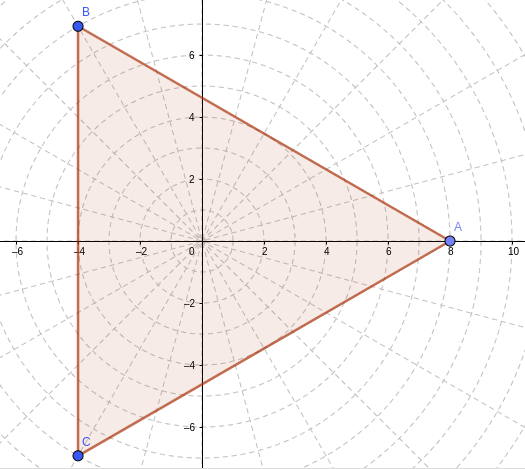
\includegraphics[width=10cm]{Gra-Ej-9.png}
\end{center}

\textcolor{ao(english)}{(\,10\,)} $\bf{\sqrt[6]{-\,27\,i}}$\\

\textcolor{ao(english)}{(\,11\,)} $\bf{\sqrt{4\,\sqrt{2}\,+\,i\,4\,\sqrt{2}}}$\\

\textcolor{ao(english)}{\ding{47}} Hallar el módulo y el angulo $\bf{z_{0}}$

$$z_{0}\,=\,4\,\sqrt{2}\,+\,i\,4\,\sqrt{2}$$

\textcolor{ao(english)}{\ding{46}} Módulo de $\bf{z_{0}}$

$$r_{0}\,=\,|z_{0}|\,=\,\sqrt{\left(4\,\sqrt{2}\right)^{2}\,+\,\left(4\,\sqrt{2}\right)^{2}}\,=\,\sqrt{16\,(2)\,+\,16\,(2)}\,=\,\sqrt{32\,+\,32}\,=\,\sqrt{64}\,=\,8$$

\textcolor{ao(english)}{\ding{46}} Angulo de $\bf{z_{0}}$

$$\theta_{0}\,=\,\tan^{-\,1}\,\left(\dfrac{4\,\sqrt{2}}{4\,\sqrt{2}}\right)\,=\,\tan^{-\,1}\,1\,=\,\dfrac{\pi}{4}$$

\textcolor{ao(english)}{\ding{47}} En este caso $\bf{n\,=\,2}$ y $\bf{k\,=\,0\,,\,1}$\\

\textcolor{ao(english)}{\ding{46}} Si $\bf{k\,=\,0}$

$$C_{0}\,=\,\sqrt{8}\,\cdot\,\,exp\,\left\{i\,\left(\dfrac{\dfrac{\pi}{4}\,+\,2\,\pi\,(0)}{2}\right)\right\}\,=\,2\,\sqrt{2}\,\cdot\,\,exp\,\left\{i\,\left(\dfrac{\dfrac{\pi}{4}}{2}\right)\right\}$$

$$C_{0}\,=\,2\,\sqrt{2}\,\cdot\,\,exp\,\left\{i\,\left(\dfrac{\pi}{8}\right)\right\}$$

$$\dfrac{\pi}{8} \quad\iff\quad 22.5^\circ$$

\textcolor{ao(english)}{\ding{46}} Si $\bf{k\,=\,1}$

$$C_{1}\,=\,\sqrt{8}\,\cdot\,\,exp\,\left\{i\,\left(\dfrac{\dfrac{\pi}{4}\,+\,2\,\pi\,(1)}{2}\right)\right\}\,=\,2\,\sqrt{2}\,\cdot\,\,exp\,\left\{i\,\left(\dfrac{\dfrac{\pi}{4}\,+\,2\,\pi}{2}\right)\right\}$$

$$=\,2\,\sqrt{2}\,\cdot\,\,exp\,\left\{i\,\left(\dfrac{\dfrac{\pi\,+\,8\,\pi}{4}}{2}\right)\right\}\,=\,2\,\sqrt{2}\,\cdot\,\,exp\,\left\{i\,\left(\dfrac{\dfrac{9\,\pi}{4}}{2}\right)\right\}$$

$$C_{1}\,=\,2\,\sqrt{2}\,\cdot\,\,exp\,\left\{i\,\left(\dfrac{9\,\pi}{8}\right)\right\}$$

$$\dfrac{9\,\pi}{8} \quad\iff\quad 202.5^\circ$$

\textcolor{ao(english)}{\ding{47}} Graficar las raices

\begin{center}
    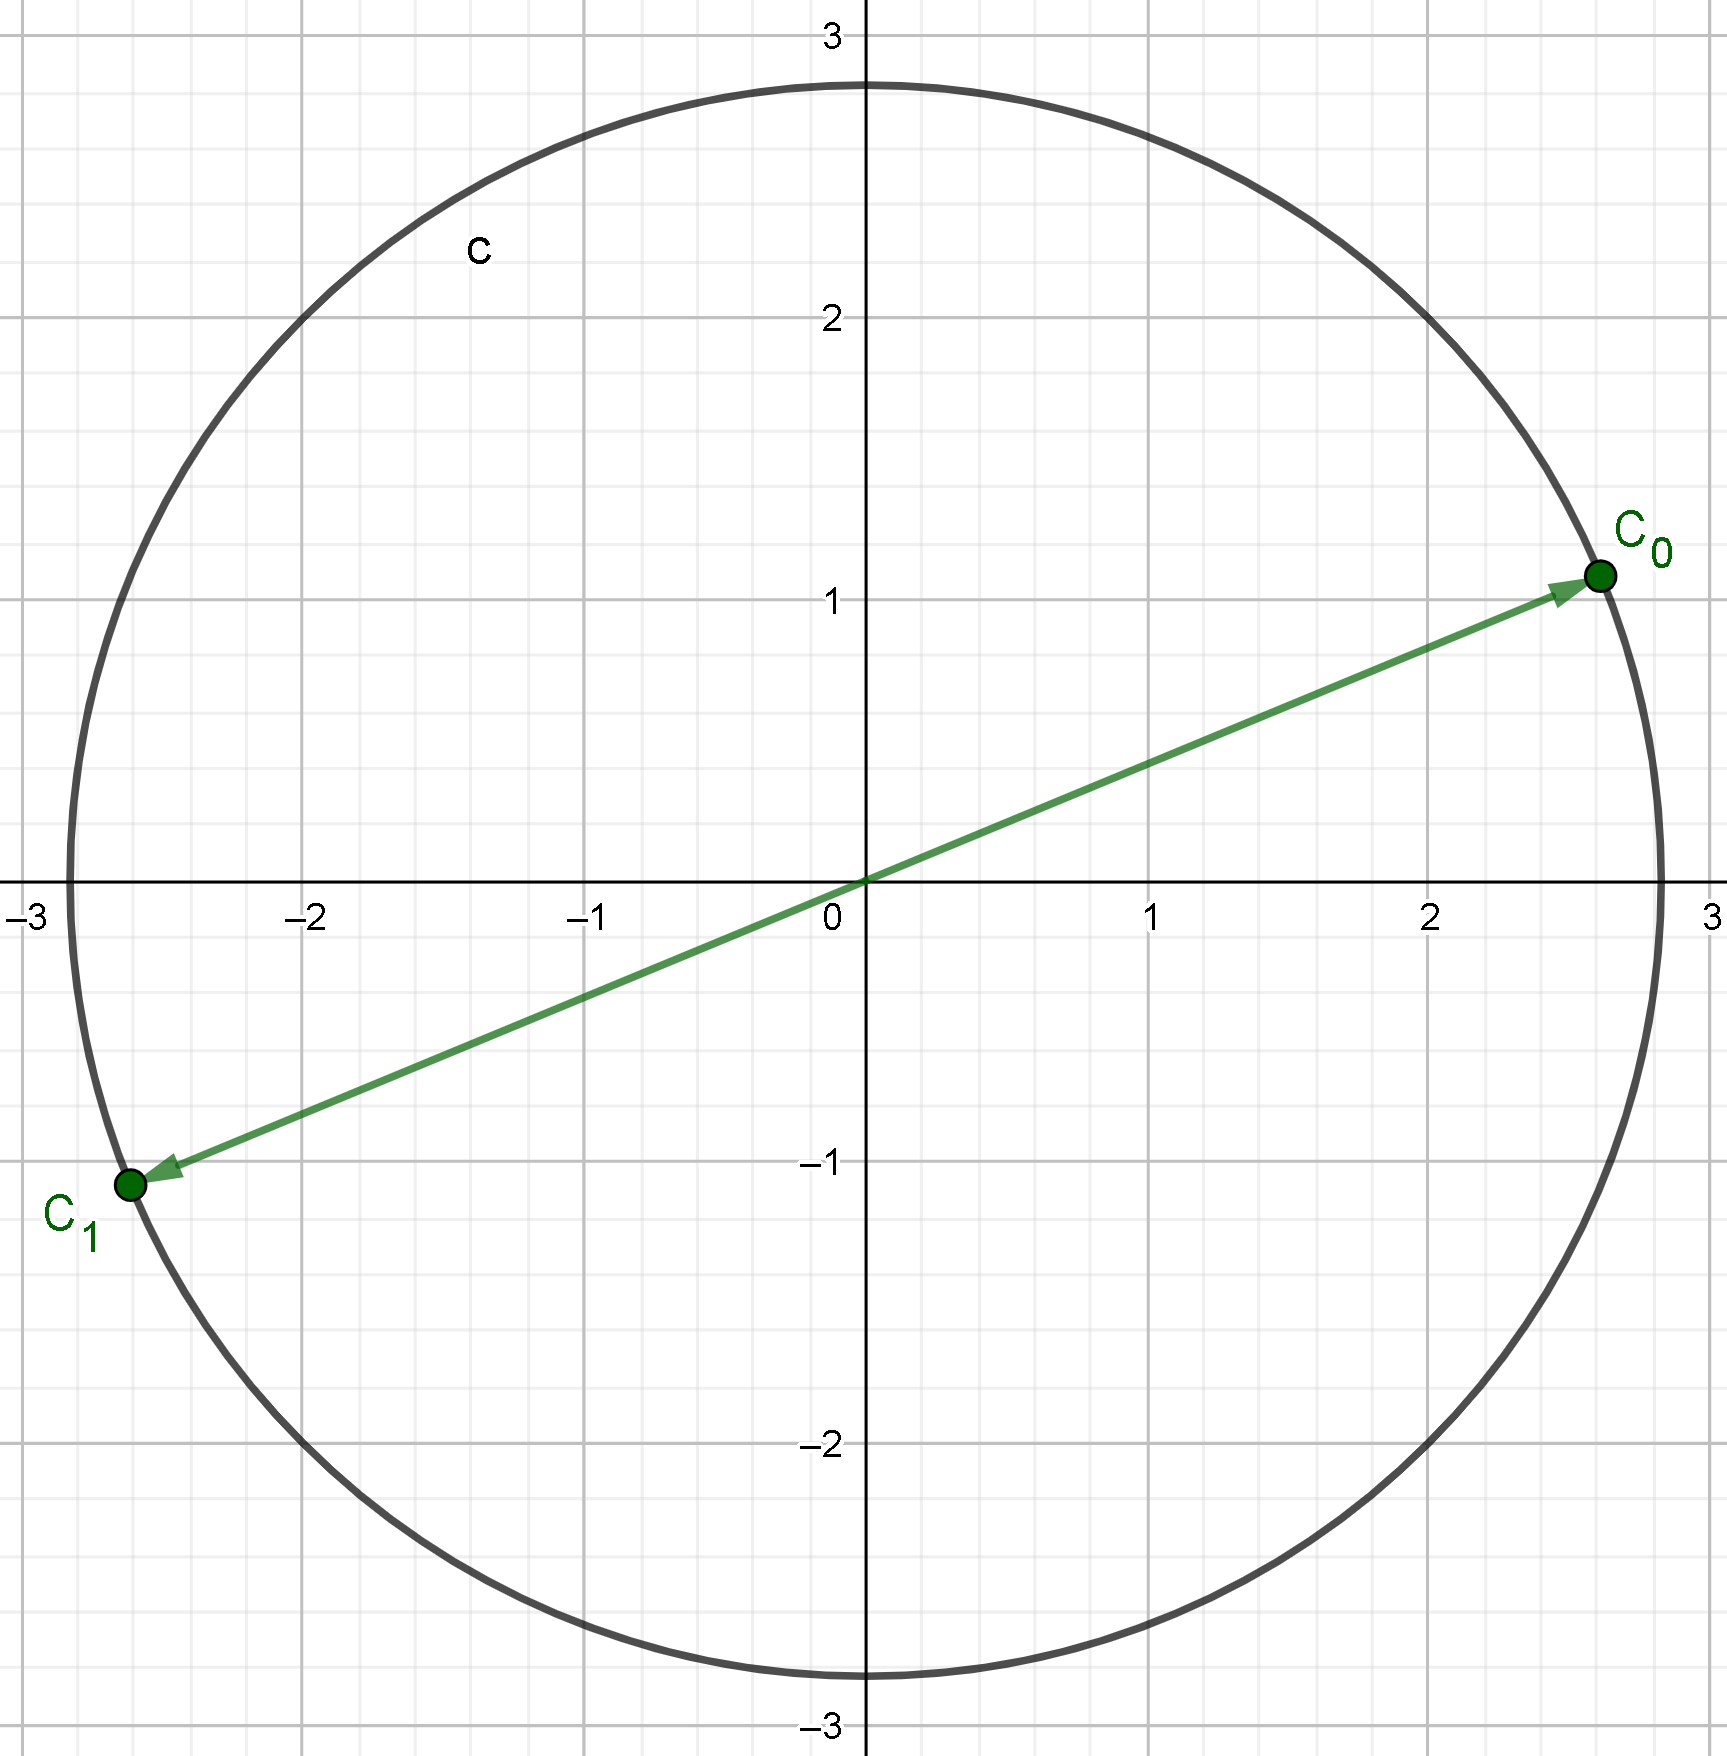
\includegraphics[width=10cm]{Gra-Ej-11.png}
\end{center}

\textcolor{ao(english)}{(\,12\,)} $\bf{\left(-\,16\,+\,i\,16\,\sqrt{3}\right)^{1\,/\,5}}$\\


\textcolor{ao(english)}{\ding{47}} Hallar el módulo y el angulo $\bf{z_{0}}$

$$z_{0}\,=\,-\,16\,+\,i\,16\,\sqrt{3}$$

\textcolor{ao(english)}{\ding{46}} Módulo de $\bf{z_{0}}$

$$r_{0}\,=\,|z_{0}|\,=\,\sqrt{\left(-\,16\right)^{2}\,+\,\left(16\,\sqrt{3}\right)^{2}}\,=\,\sqrt{256\,+\,256\,\left(3\right)}\,=\,\sqrt{1024}\,=\,32$$

\textcolor{ao(english)}{\ding{46}} Angulo de $\bf{z_{0}}$

$$\theta_{0}\,=\,\tan^{-\,1}\,\left(\dfrac{16\,\sqrt{3}}{-\,16}\right)\,=\,\tan^{-\,1}\,\left(-\,\sqrt{3}\right)\,=\,-\,\dfrac{\pi}{3}$$

\textcolor{ao(english)}{\ding{43}} Correción $\theta_{0}$ Cuadrantre II

$$\theta_{2}\,=\,\pi\,-\,|\theta_{0}|\,=\,\pi\,-\,\left|-\,\dfrac{\pi}{3}\right|\,=\,\pi\,-\,\dfrac{\pi}{3}\,=\,\dfrac{3\,\pi\,-\,\pi}{3}\,=\,\dfrac{2\,\pi}{3}$$

\textcolor{ao(english)}{\ding{47}} En este caso $\bf{n\,=\,5}$ y $\bf{k\,=\,0\,,\,1\,,\,2\,,3\,,4}$\\

\textcolor{ao(english)}{\ding{46}} Si $\bf{k\,=\,0}$
$$C_{0}\,=\,32\,\cdot\,\,exp\,\left\{i\,\left(\dfrac{\dfrac{2\,\pi}{3}\,+\,2\,\pi\,(0)}{5}\right)\right\}\,=\,32\,\cdot\,\,exp\,\left\{i\,\left(\dfrac{\dfrac{2\,\pi}{3}\,+\,0}{5}\right)\right\}$$

$$=\,32\,\cdot\,\,exp\,\left\{i\,\left(\dfrac{\dfrac{2\,\pi}{3}}{5}\right)\right\}$$

$$C_{0}\,=\,32\,\cdot\,\,exp\,\left\{i\,\left(\dfrac{2\,\pi}{15}\right)\right\}$$

$$\dfrac{2\,\pi}{15} \quad\iff\quad 24^\circ$$

\textcolor{ao(english)}{\ding{46}} Si $\bf{k\,=\,1}$
$$C_{1}\,=\,32\,\cdot\,\,exp\,\left\{i\,\left(\dfrac{\dfrac{2\,\pi}{3}\,+\,2\,\pi\,(1)}{5}\right)\right\}\,=\,32\,\cdot\,\,exp\,\left\{i\,\left(\dfrac{\dfrac{2\,\pi}{3}\,+\,2\,\pi}{5}\right)\right\}$$

$$=\,32\,\cdot\,\,exp\,\left\{i\,\left(\dfrac{\dfrac{2\,\pi\,+\,6\,\pi}{3}}{5}\right)\right\}=\,32\,\cdot\,\,exp\,\left\{i\,\left(\dfrac{\dfrac{8\,\pi}{3}}{5}\right)\right\}$$

$$C_{1}\,=\,32\,\cdot\,\,exp\,\left\{i\,\left(\dfrac{8\,\pi}{15}\right)\right\}$$

$$\dfrac{8\,\pi}{15} \quad\iff\quad 96^\circ$$

\textcolor{ao(english)}{\ding{46}} Si $\bf{k\,=\,2}$
$$C_{2}\,=\,32\,\cdot\,\,exp\,\left\{i\,\left(\dfrac{\dfrac{2\,\pi}{3}\,+\,2\,\pi\,(2)}{5}\right)\right\}\,=\,32\,\cdot\,\,exp\,\left\{i\,\left(\dfrac{\dfrac{2\,\pi}{3}\,+\,4\,\pi}{5}\right)\right\}$$

$$=\,32\,\cdot\,\,exp\,\left\{i\,\left(\dfrac{\dfrac{2\,\pi\,+\,12\,\pi}{3}}{5}\right)\right\}=\,32\,\cdot\,\,exp\,\left\{i\,\left(\dfrac{\dfrac{14\,\pi}{3}}{5}\right)\right\}$$

$$C_{2}\,=\,32\,\cdot\,\,exp\,\left\{i\,\left(\dfrac{14\,\pi}{15}\right)\right\}$$

$$\dfrac{14\,\pi}{15} \quad\iff\quad 168^\circ$$

\textcolor{ao(english)}{\ding{46}} Si $\bf{k\,=\,3}$
$$C_{3}\,=\,32\,\cdot\,\,exp\,\left\{i\,\left(\dfrac{\dfrac{2\,\pi}{3}\,+\,2\,\pi\,(3)}{5}\right)\right\}\,=\,32\,\cdot\,\,exp\,\left\{i\,\left(\dfrac{\dfrac{2\,\pi}{3}\,+\,6\,\pi}{5}\right)\right\}$$

$$=\,32\,\cdot\,\,exp\,\left\{i\,\left(\dfrac{\dfrac{2\,\pi\,+\,18\,\pi}{3}}{5}\right)\right\}=\,32\,\cdot\,\,exp\,\left\{i\,\left(\dfrac{\dfrac{20\,\pi}{3}}{5}\right)\right\}$$

$$C_{3}\,=\,32\,\cdot\,\,exp\,\left\{i\,\left(\dfrac{20\,\pi}{15}\right)\right\}\,=\,32\,\cdot\,\,exp\,\left\{i\,\left(\dfrac{4\,\pi}{3}\right)\right\}$$

$$\dfrac{4\,\pi}{3} \quad\iff\quad 240^\circ$$

\textcolor{ao(english)}{\ding{46}} Si $\bf{k\,=\,4}$
$$C_{4}\,=\,32\,\cdot\,\,exp\,\left\{i\,\left(\dfrac{\dfrac{2\,\pi}{3}\,+\,2\,\pi\,(4)}{5}\right)\right\}\,=\,32\,\cdot\,\,exp\,\left\{i\,\left(\dfrac{\dfrac{2\,\pi}{3}\,+\,8\,\pi}{5}\right)\right\}$$

$$=\,32\,\cdot\,\,exp\,\left\{i\,\left(\dfrac{\dfrac{2\,\pi\,+\,24\,\pi}{3}}{5}\right)\right\}=\,32\,\cdot\,\,exp\,\left\{i\,\left(\dfrac{\dfrac{26\,\pi}{3}}{5}\right)\right\}$$

$$C_{4}\,=\,32\,\cdot\,\,exp\,\left\{i\,\left(\dfrac{26\,\pi}{15}\right)\right\}$$

$$\dfrac{26\,\pi}{15} \quad\iff\quad 312^\circ$$

\textcolor{ao(english)}{\ding{47}} Graficar las raices

\begin{center}
    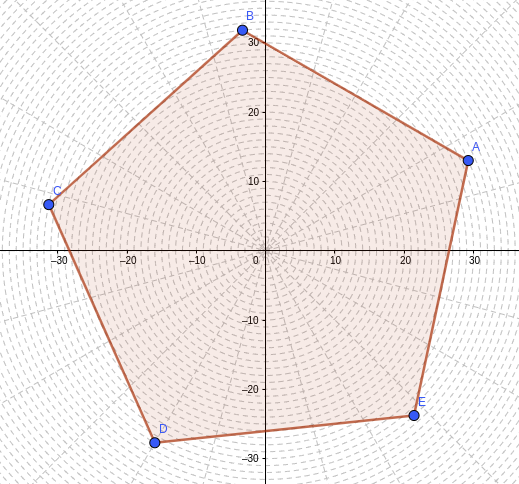
\includegraphics[width=10cm]{Gra-Ej-12.png}
\end{center}

\end{document}